\section{Position de la voiture dans l'image}
\begin{enumerate}
  \item \q{Par la méthode de votre choix, écrire une fonction qui retourne les
          coordonnées (X,Y) en pixels du centre de la voiture par rapport au centre de
          l'image.}
        \codeFromFileT{helpers/image.py}{section-04/q1-1.py}
        \codeFromFileT{main.py}{section-04/q1-2.py}
        \ul{Remarque :} Cette fois-ci j'utilise \il{plt} et non mon \il{Plotter}
        car il ne peut pas afficher des listes de points...\\
        Et j'obtiens l'image de gauche que j'ai agrandi à droite.
        \begin{center}
          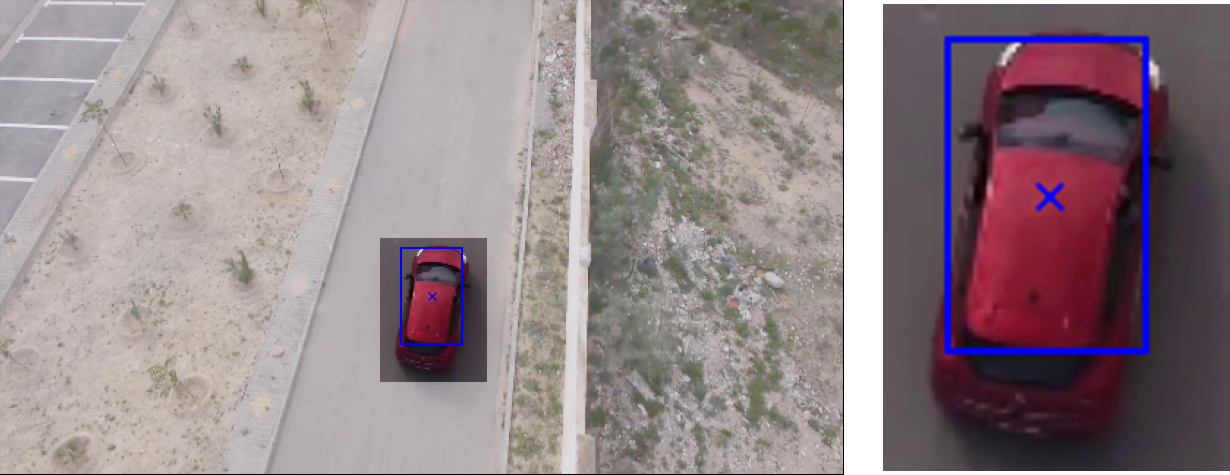
\includegraphics[scale=0.25]{section-04/q1-3.png}
        \end{center}
\end{enumerate}
